%%%%%%%%%%%%%%%%%%%%%%%%%%%%%%%%%%%%%%%%%
% Plasmati Graduate CV
% LaTeX Template
% Version 1.0 (24/3/13)
%
% This template has been downloaded from:
% http://www.LaTeXTemplates.com
%
% Original author:
% Alessandro Plasmati (alessandro.plasmati@gmail.com)
%
% License:
% CC BY-NC-SA 3.0 (http://creativecommons.org/licenses/by-nc-sa/3.0/)
%
% Important note:
% This template needs to be compiled with XeLaTeX.
% The main document font is called Fontin and can be downloaded for free
% from here: http://www.exljbris.com/fontin.html
%
%%%%%%%%%%%%%%%%%%%%%%%%%%%%%%%%%%%%%%%%%

%----------------------------------------------------------------------------------------
%	PACKAGES AND OTHER DOCUMENT CONFIGURATIONS
%----------------------------------------------------------------------------------------

\documentclass[a4paper,10pt]{article} % Default font size and paper size

\usepackage{fontspec} % For loading fonts
\defaultfontfeatures{Mapping=tex-text}
\setmainfont[SmallCapsFont = Fontin SmallCaps]{Fontin} % Main document font

\usepackage{xunicode,xltxtra,url,parskip} % Formatting packages

\usepackage[usenames,dvipsnames]{xcolor} % Required for specifying custom colors
\usepackage{comment}
\usepackage[big]{layaureo} % Margin formatting of the A4 page, an alternative to layaureo can be \usepackage{fullpage}
% To reduce the height of the top margin uncomment: \addtolength{\voffset}{-1.3cm}
\usepackage{textcomp}
\usepackage{hyperref} % Required for adding links	and customizing them
\definecolor{linkcolour}{rgb}{0,0.2,0.6} % Link color
\hypersetup{colorlinks,breaklinks,urlcolor=linkcolour,linkcolor=linkcolour} % Set link colors throughout the document
\usepackage[some]{background}
\backgroundsetup{contents={
\includegraphics[width=0.2\textwidth]{images/durham.png}},scale=1,placement=top,opacity=0.13,position={14.5cm,-.3cm}}

\usepackage{titlesec} % Used to customize the \section command
\titleformat{\section}{\large\scshape\raggedright}{}{0em}{}[\titlerule] % Text formatting of sections
\titleformat{\subsection}{\bfseries\normalsize\slshape\raggedright}{}{0em}{}[] % Text formatting of sections
\titlespacing{\section}{0pt}{1.5pt}{1.5pt} % Spacing around sections
\titlespacing{\subsection}{0pt}{1.5pt}{1.5pt} % Spacing around sections


\addtolength{\oddsidemargin}{-.8cm}
\addtolength{\evensidemargin}{-.8cm}
\addtolength{\textwidth}{1.75cm}
\addtolength{\topmargin}{-1cm}
\addtolength{\textheight}{1.75cm}

\begin{document}

\pagestyle{empty} % Removes page numbering
\BgThispage
\font\fb=''[cmr10]'' % Change the font of the \LaTeX command under the skills section

\small
%----------------------------------------------------------------------------------------
%	NAME AND CONTACT INFORMATION
%----------------------------------------------------------------------------------------

% No-photo on the top

%\par{\centering{\huge \textsc{Uzmar de Jesús Gómez Yáñez}}\bigskip\par} % Your name
%\par{\centering{\Large \textsc{Curriculum Vitae}}\bigskip\par}


%Photo on the top
% \par{\centering{\huge \textsc{\hspace{2cm}Uzmar de Jesús Gómez Yáñez}}\bigskip\par} % Your name
% \par{\centering{\Large \textsc{\hspace{2cm}Curriculum Vitae}}\bigskip\par}
% \smash{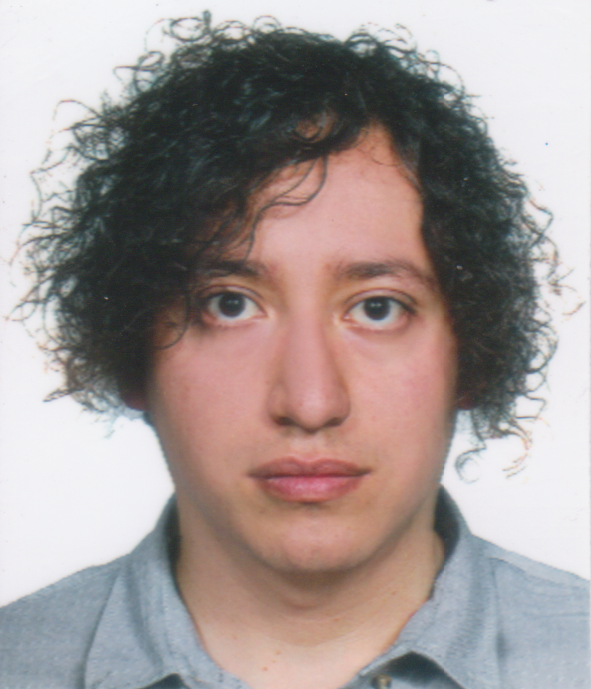
\includegraphics[width=2.5cm]{images/fotoinfantil.png}}
% \par{\centering{\large \textsc{\hspace{2cm}
% 			{\color{brown}MSc Scientific Computing and Data Analysis}}}\bigskip\par}

%Without photo
\par{\centering{\huge \textsc{Uzmar de Jesús Gómez Yáñez}}\bigskip\par} % Your name
\par{\centering{\Large \textsc{Curriculum Vitae}}\bigskip\par}
\par{\centering{\large \textsc{
			{\color{brown}MSc Scientific Computing and Data Analysis}}}\bigskip\par}


\bigskip
\section{Personal Statement}
\bigskip
Hands-on experience applying Machine Learning algorithms. Excellent usage of GNU / Linux systems and knowledge of object-oriented programming languages such as Python and C++. I have worked in the academic field as a teacher assistant, teaching mathematics, computer science, physics and other topics at a university level. Good understanding of algorithms, data structures, bayesian statistics, etc. Experience managing containerized applications using Kubernetes.

\bigskip
\section{Personal Data}
\bigskip
\begin{tabular}{rl}
%\textsc{Place and Date of Birth:} & Mexico | September 25, 1992 \\
\textsc{Address:} & London, England \\
\textsc{Phone:} & +44 7704 613361\\
\textsc{email:} & \href{mailto:uzmar.gomez@hotmail.com}{uzmar.gomez@hotmail.com}\\
\textsc{LinkedIn:} & \href{www.linkedin.com}{www.linkedin.com/in/uzmargomez}\\
\textsc{Github:} & \href{https://github.com/uzmargomez}{https://github.com/uzmargomez}%\\
%\textsc{HackerRank:} & \href{https://www.hackerrank.com/uzmar_gomez}{https://www.hackerrank.com/uzmar\_gomez}
\end{tabular}

%----------------------------------------------------------------------------------------
%	EDUCATION
%----------------------------------------------------------------------------------------
\bigskip
\section{Education}
\bigskip
\begin{tabular}{r|p{14.5cm}}	
	
	%------------------------------------------------	
	\textsc{Present} & \textbf{MSc in Scientific Computing and Data Analysis}, Department of Computer Science, Durham University, \small Durham, United Kingdom.\\
	\textsc{2021} & Specialization: Earth and Environmental Sciences\\
	& Dissertation: \emph{``GPU Programming with Standard C++''}\\ 
	& \small Description: We used NVIDIA HPC SDK compiler suite to accelerate ExaHyPE's Finite Volume scheme, a\\
	&\hspace{1.7cm} \small generic code base to simulate wave equations. The resulting code was benchmarked against\\
	&\hspace{1.7cm} an OpenMP GPU offloading code port of exactly the same code structure, and we report on some\\
	&\hspace{1.7cm} problems and benefits of the new C++ software stack.\\
	& \small Advisor: Dr. Tobias Weinzierl\\
	& \\
	&\normalsize \textsc{Grade}: Distinction\hyperlink{grdsmsc}{\hfill | \footnotesize Detailed List of Grades}\\
	\multicolumn{2}{c}{}\\

%------------------------------------------------	
	
	\textsc{2018} & \textbf{BSc in Physics}, Faculty of Science, National Autonomous University of Mexico (UNAM), \small Mexico City, Mexico.\\
	\textsc{2011} & Dissertation: \emph{``Numerical Study of Vlasov Equation in the Schwarzschild Metric''}\\
	&\small Description: Creation of a finite differences scheme that evolves the relativistic Vlasov equation on a\\
	&\hspace{1.7cm} \small black hole metric background, assuming this is an advective equation, with velocities \\
	&\hspace{1.7cm} \small dependent both on time and position.\\
	& \small Advisor: Dr. Miguel Alcubierre\\
	& \\
	&\normalsize \textsc{Overall Score}: 9.37/10\hyperlink{grdsbach}{\hfill | \footnotesize Detailed List of Grades}\\
	\multicolumn{2}{c}{}\\
	
%------------------------------------------------
	
\end{tabular}

%----------------------------------------------------------------------------------------
%	LANGUAGES
%----------------------------------------------------------------------------------------
\section{Languages}
\bigskip
\begin{tabular}{rl}
	\textsc{English:} & C1 Level - IELTS (2021)\\
	\textsc{Spanish:} & Mothertongue \\
	\textsc{French:} & Basic
\end{tabular}


%----------------------------------------------------------------------------------------
%	COMPUTER SKILLS 
%----------------------------------------------------------------------------------------

\section{Computer Skills}
\bigskip
\begin{tabular}{r|p{10.5cm}}
	Programming Languages & Python, C++, Fortran, Julia \\
	Machine/Deep Learning & TensorFlow, Keras, PyTorch, Facebook Prophet, ARIMA, SARIMA, LDA, PCA, Kmeans, KNN, Neural Networks, Recommendation systems, Classification and Regression problems\\
	Serving & Triton, Seldon Core, TFServing \\
	Databases & SQL, MongoDB \\
	Containers & Docker, Kubernetes \\
	Operating Systems & GNU/Linux, Windows \\
	Web Backend & Flask \\
	Web Frontend & HTML (Plotly Dash), Bootstrap \\
	Version Control & Git \\
	Parallel Computing & C++ Standard Algorithms, CUDA Python\\
	Data Visualization & Plotly Dash, Qlik, Tableau \\
	GCP Tools & BigQuery, BQ ML, Compute Engine, Composer, Artifact Registry, Kubernetes Engine, Storage, Data Studio, Kubeflow, Data Fusion, Cloud Build, VertexAI
	%	\multicolumn{2}{c}{} \\
\end{tabular}
\bigskip

%----------------------------------------------------------------------------------------
%	WORK EXPERIENCE 
%----------------------------------------------------------------------------------------

\section{Experience}
\bigskip

\subsection{Short Description}
\vspace{0.2cm}
\textbf{Sep 2022 - Present}. Associate ML Research and Development Programmer at Rockstar Games. 

\textbf{Jul 2020 - Jan 2022}. Data Scientist at Rackspace Technology. I helped on the migration of data from on-premises servers to the GCP cloud. I worked on churn prediction models that used features related to the COVID19 spreading aside from other business-related features to predict customer attrition, this work includes the development of the model using XGBoost, as well as the deployment of it using Kubeflow and the serving via Seldon Core. I was also involved in constructing an SSAS OLAP Cube to be used by the company for inventory-related queries. I worked on NLP tasks, such as the extraction of themes out of tickets using semantic similarity, by getting embeddings vectors out of sentences with a transformer architecture named Universal Sentence Encoder. Worked on how to translate voice to text. I built two production-level applications using Plotly Dash.

\textbf{Dec 2019 - Jun 2020}. Data Scientist at Softtek. I worked on a face recognition system using a method called Sparse Representation and another one using Neural Networks. I acquired a deep understanding of Neural Networks for Face Detection and Recognition, Image Classification, Language Processing, among others, as well as some experience in Data Visualization tools such as Tableau.

\textbf{Sep 2019 - Dec 2019}. Data Scientist Trainee at Softtek. I learned about different statistical and machine learning techniques, as well as algorithms, to study a wide variety of problems.

\textbf{Sep 2018 - Dec 2019}. I have research experience using the Einstein Toolkit, a software platform created for supporting research in relativistic astrophysics and gravitational physics.

\textbf{2016 - 2019}. Worked as a Teacher assistant. I've given lectures aimed to Computer Science and Physics Students in the following topics:
\begin{itemize}
	\item Computer Science.
	
	\href{https://web.fciencias.unam.mx/asignaturas/102.pdf}{https://web.fciencias.unam.mx/asignaturas/102.pdf}
	
	\item Selected Topics in Relativity, Cosmology and Gravitation 1.
	
	\href{https://web.fciencias.unam.mx/docencia/horarios/presentacion/295997}{https://web.fciencias.unam.mx/docencia/horarios/presentacion/295997}
	
	\item Relativity
	
	\href{https://web.fciencias.unam.mx/asignaturas/718.pdf}{https://web.fciencias.unam.mx/asignaturas/718.pdf}
	
	\item Mathematics I for Applied Sciences. 
	
	\href{http://www.fciencias.unam.mx/asignaturas/1118.pdf}{http://www.fciencias.unam.mx/asignaturas/1118.pdf}
	
	\item Mathematics II for Applied Sciences.
	
	\href{http://www.fciencias.unam.mx/asignaturas/1216.pdf}{http://www.fciencias.unam.mx/asignaturas/1216.pdf}
\end{itemize}
\bigskip

%----------------------------------------------------------------------------------------
%	INTERESTS AND ACTIVITIES
%----------------------------------------------------------------------------------------

\section{Interests and Activities}
\bigskip
\subsection*{Academic}
Data Science, Machine Learning, Deep Learning, Numerical Analysis, General Relativity, Numerical Relativity, Black Holes.
\subsection*{Non academic}
Science Fiction and Fantasy Reading, Videogames, Running, Swimming, Playing Guitar, Traveling. 
\bigskip

%----------------------------------------------------------------------------------------
%	EXTRA CURRICULAR ACTIVITIES
%---------------------------------------------------------------------------------------

\section{Extra Curricular Activities}
\bigskip
\begin{tabular}{r|p{11cm}}
	\textsc{Jun 2022} & Student Representative MiSCaDA Programme\\
	\textsc{Oct 2021}&\footnotesize{\textbf{Durham University}}\\
	&\footnotesize{Provide a link between students and the University Staff. Sit on the Student/Staff Comittee to discuss issues within the department raised by the students}\\
	\multicolumn{2}{c}{} \\
\end{tabular}

\begin{comment}
\vspace{0.4cm}
\subsection*{Technical}
\vspace{0.2cm}
\begin{tabular}{r|p{11cm}}

	\textsc{Present}& Associate ML Research and Development Programmer at \textsc{Rockstar Games}\\
	\textsc{Sep 2022}& \small London, United Kingdom.\\
	\multicolumn{2}{c}{} \\
	
	%------------------------------------------------

	\textsc{Jan 2022}& Data Scientist II at \textsc{Rackspace Technology}\\
	\textsc{Aug 2021}& \small Mexico City, Mexico.\\
	\multicolumn{2}{c}{} \\
	
	%------------------------------------------------

	\textsc{Aug 2021}& Data Scientist I at \textsc{Rackspace Technology}\\
	\textsc{Jul 2020}& \small Mexico City, Mexico.\\
	\multicolumn{2}{c}{} \\
	
	%------------------------------------------------
	
	\textsc{Jun 2020}& Data Scientist at \textsc{Softtek}\\
	\textsc{Jan 2020}& \small Mexico City, Mexico.\\
	\multicolumn{2}{c}{} \\
	
	%------------------------------------------------
	
	\textsc{Dec 2019}& Data Scientist Trainee at \textsc{Softtek}\\
	\textsc{Sep 2019}& \small Mexico City, Mexico.\\
	\multicolumn{2}{c}{} \\
	
	%------------------------------------------------
	
\end{tabular}

\subsection*{Vocational}
\begin{tabular}{r|p{7.8cm}p{4cm}}
%------------------------------------------------

Semester 2019-2 & Teacher Assistant B at \textsc{Faculty of Science, UNAM} &\\
& \small Mexico City, Mexico. & \\
& \footnotesize $\circ$ Mathematics II for Applied Sciences & | {\footnotesize MSc. Alejandro Villarreal}\\
\multicolumn{3}{c}{} \\

%------------------------------------------------

Semester 2019-1 & Teacher Assistant B at \textsc{Faculty of Science, UNAM} &\\
& \small Mexico City, Mexico. & \\
& \footnotesize $\circ$ Selected Topics in Relativity, Cosmology and Gravitation I & | {\footnotesize Dr. Miguel Alcubierre}\\
& \footnotesize $\circ$ Mathematics I for Applied Sciences & | {\footnotesize MSc. Alejandro Villarreal}\\
\multicolumn{3}{c}{} \\

%------------------------------------------------

Semester 2018-2 & Teacher Assistant B at \textsc{Faculty of Science, UNAM} &\\
& \small Mexico City, Mexico. & \\
& \footnotesize $\circ$ Relativity & | {\footnotesize Dr. Miguel Alcubierre}\\
& \footnotesize $\circ$ Mathematics II for Applied Sciences & | {\footnotesize MSc. Alejandro Villarreal}\\
\multicolumn{3}{c}{} \\

%------------------------------------------------

Semester 2018-1 & Teacher Assistant B at \textsc{Faculty of Science, UNAM} &\\
&\small Mexico City, Mexico. & \\
& \footnotesize $\circ$ Relativity & | {\footnotesize Dr. Miguel Alcubierre}\\
& \footnotesize $\circ$ Mathematics I for Applied Sciences & | {\footnotesize MSc. Alejandro Villarreal}\\
\multicolumn{3}{c}{} \\

%------------------------------------------------
\end{tabular}

\begin{tabular}{r|p{7.8cm}p{4cm}}
Semester 2017-2 & Teacher Assistant A at \textsc{Faculty of Science, UNAM} &\\
&\small Mexico City, Mexico. & \\
& \footnotesize $\circ$ Mathematics II for Applied Sciences & | {\footnotesize MSc. Alejandro Villarreal}\\
\multicolumn{3}{c}{} \\

%------------------------------------------------

Semester 2017-1 & Teacher Assistant A at \textsc{Faculty of Science, UNAM} &\\
&\small Mexico City, Mexico. & \\
& \footnotesize $\circ$ Mathematics I for Applied Sciences & | {\footnotesize MSc. Alejandro Villarreal}\\
& \footnotesize $\circ$ Computer Science & | {\footnotesize MSc. Alejandro Villarreal}\\
\multicolumn{3}{c}{} \\

%------------------------------------------------

\textsc{Jun 2017} & Teacher at \textsc{Coordination of Programs of Differentiated Attention for Students, Faculty of Engineering, UNAM} &\\
& \small Mexico City, Mexico. & \\
& \footnotesize $\circ$ Electrodynamics with an introduction to special relativity & | {\footnotesize Eng. Raúl Puente}\\
\multicolumn{3}{c}{} \\

%------------------------------------------------

Semester 2016-1 & Teacher Assistant A at \textsc{Faculty of Science, UNAM} &\\
& \small Mexico City, Mexico. & \\
& \footnotesize $\circ$ Mathematics I for Applied Sciences & | {\footnotesize MSc. Alejandro Villarreal}\\
\multicolumn{3}{c}{} \\
%------------------------------------------------
\end{tabular}

%----------------------------------------------------------------------------------------
%	CONFERENCES, SUMMER SCHOOLS AND WORKSHOPS ASSISTED
%----------------------------------------------------------------------------------------
\bigskip
\section{Conferences, Courses, Schools and Workshops Attended}
\bigskip
\subsection*{Computer Science Related}

\begin{tabular}{r|p{11cm}}

	%------------------------------------------------
		
	% \textsc{Present} & \small \textbf{Specialization}. \textit{TensorFlow in Practice} (COURSERA)\\
	% \textsc{Jun 15, 2020} & \small DeepLearning.ai\\
	% &\url{}\\
	% \multicolumn{2}{c}{} \\

	%------------------------------------------------
		
	% \textsc{Present} & \small \textbf{Course}. \textit{Sequences, Time Series and Prediction} (COURSERA)\\
	% \textsc{Jun 15, 2020} & \small DeepLearning.ai\\
	% &\url{}\\
	% \multicolumn{2}{c}{} \\

	%------------------------------------------------
			
	% \textsc{Present} & \small \textbf{Course}. \textit{Natural Language Processing in TensorFlow} (COURSERA)\\
	% \textsc{Jun 19, 2020} & \small DeepLearning.ai\\
	% &\url{}\\
	% \multicolumn{2}{c}{} \\

	%------------------------------------------------
			
	% \textsc{Jun 29, 2020} & \small \textbf{Course}. \textit{SQL for Data Science} (COURSERA)\\
	% \textsc{Jun 27, 2020} & \small University of California, Davis\\
	% &\url{}\\
	% \multicolumn{2}{c}{} \\

	\textsc{Sep 02, 2021} & \small \textbf{Course}. \textit{Probability - The Science of Uncertainty and Data}\\
	\textsc{May 03, 2021} & \small MITx on edX\\
	&\url{https://courses.edx.org/certificates/77ed32f3abc34158896ab5f2ee6d18be}\\
	\multicolumn{2}{c}{} \\

	\textsc{Oct 09, 2020} & \small \textbf{Conference}. \textit{THE Data Science Conference}\\
	\textsc{Oct 08, 2020} & \small Online conference due to COVID19\\
	&\url{https://www.thedatascienceconference.com}\\
	\multicolumn{2}{c}{} \\

	%------------------------------------------------

	\textsc{Oct 09, 2020} & \small \textbf{Course}. \textit{Building Resilient Streaming Analytics Systems on GCP} (COURSERA)\\
	\textsc{Oct 08, 2020} & \small Google Cloud Platform\\
	&\url{https://www.coursera.org/account/accomplishments/certificate/ZNG729Z9L78P}\\
	\multicolumn{2}{c}{} \\
				
		
	%------------------------------------------------

	\textsc{Oct 08, 2020} & \small \textbf{Course}. \textit{Modernizing Data Lakes and Data Warehouses with GCP} (COURSERA)\\
	\textsc{Oct 07, 2020} & \small Google Cloud Platform\\
	&\url{https://www.coursera.org/account/accomplishments/certificate/JUDDNMKRSBUA}\\
	\multicolumn{2}{c}{} \\

\end{tabular}

\begin{tabular}{r|p{11cm}}

	%------------------------------------------------
	
	\textsc{Oct 07, 2020} & \small \textbf{Course}. \textit{Building Batch Data Pipelines on GCP} (COURSERA)\\
	\textsc{Sep 10, 2020} & \small Google Cloud Platform\\
	&\url{https://www.coursera.org/account/accomplishments/certificate/8KTYPM3GZQS7}\\
	\multicolumn{2}{c}{} \\
	%------------------------------------------------	

	\textsc{Sep 10, 2020} & \small \textbf{Course}. \textit{Smart Analytics, Machine Learning, and AI on GCP} (COURSERA)\\
	\textsc{Sep 01, 2020} & \small Google Cloud Platform\\
	&\url{https://www.coursera.org/account/accomplishments/certificate/LAZ8CNLM2M5A}\\
	\multicolumn{2}{c}{} \\
	%------------------------------------------------

	\textsc{Ago 09, 2020} & \small \textbf{Course}. \textit{Google Cloud Platform Big Data and Machine Learning Fundamentals} (COURSERA)\\
	\textsc{Ago 01, 2020} & \small Google Cloud Platform\\
	&\url{https://www.coursera.org/account/accomplishments/certificate/S9HSH92LSALR}\\
	\multicolumn{2}{c}{} \\

	%------------------------------------------------
		
		
	\textsc{Jun 19, 2020} & \small \textbf{Course}. \textit{Convolutional Neural Networks in TensorFlow} (COURSERA)\\
	\textsc{Jun 15, 2020} & \small DeepLearning.ai\\
	&\url{https://www.coursera.org/account/accomplishments/certificate/76LGX8GCUG5D}\\
	\multicolumn{2}{c}{} \\

	%------------------------------------------------
	
	\textsc{Jun 15, 2020} & \small \textbf{Course}. \textit{Introduction to TensorFlow for Artificial Intelligence, Machine Learning, and Deep Learning} (COURSERA)\\
	\textsc{Jun 15, 2020} & \small DeepLearning.ai\\
	&\url{https://www.coursera.org/account/accomplishments/certificate/LZJ2FSW2RJGP}\\
	\multicolumn{2}{c}{} \\

	%------------------------------------------------
	\textsc{May 04, 2020} & \small \textbf{Course}. \textit{AI \& Deep Learning with TensorFlow} (EDUREKA)\\
	\textsc{Mar 04, 2020} & \small Edureka! For Business\\
	&\url{https://www.edureka.co/lms/certificate/c3d0ebdc5518b429f6cc1a009454a9df}\\
	\multicolumn{2}{c}{} \\
	
	%------------------------------------------------
	
	\textsc{Mar 26, 2020} & \small \textbf{Specialization}. \textit{Accelerated Computer Science Fundamentals} (COURSERA)\\
	\textsc{Ago 04, 2019} & \small University of Illinois at Urbana-Champaign\\
	&\url{https://www.coursera.org/account/accomplishments/specialization/certificate/DRF2CVM7P7FB}\\
	\multicolumn{2}{c}{} \\
	
	%------------------------------------------------
	
	\textsc{Mar 26, 2020} & \small \textbf{Course}. \textit{Unordered Data Structures} (COURSERA)\\
	\textsc{Sep 15, 2019} & \small University of Illinois at Urbana-Champaign\\
	&\url{https://www.coursera.org/account/accomplishments/certificate/DFHE5FBHVAAD}\\
	\multicolumn{2}{c}{} \\
	
	%------------------------------------------------
	\textsc{Mar 04, 2020} & \small \textbf{Course}. \textit{Python Statistics for Data Science Course} (EDUREKA)\\
	\textsc{Feb 10, 2020} & \small Edureka! For Business\\
	&\url{https://www.edureka.co/lms/certificate/8a0976c4e21d5bee00ff053e2d8e3f3e}\\
	\multicolumn{2}{c}{} \\
	
	%------------------------------------------------

	\textsc{Sep 15, 2019} & \small \textbf{Course}. \textit{Ordered Data Structures} (COURSERA)\\
	\textsc{Ago 11, 2019} & \small University of Illinois at Urbana-Champaign\\
	&\url{https://www.coursera.org/account/accomplishments/certificate/PZ9NABHA7XBY}\\
	\multicolumn{2}{c}{} \\
	
	%------------------------------------------------
	
	\textsc{Ago 11, 2019} & \small \textbf{Course}. \textit{Object-Oriented Data Structures in C++} (COURSERA)\\
	\textsc{Ago 04, 2019} & \small University of Illinois at Urbana-Champaign\\
	&\url{https://www.coursera.org/account/accomplishments/certificate/2YKURK8TJJ5B}\\
	\multicolumn{2}{c}{} \\

	%------------------------------------------------
	
	\textsc{Jul 29, 2019} & \small \textbf{Course}. \textit{Algorithmic Toolbox} (COURSERA)\\
	\textsc{Jun 02, 2019} & \small University of California San Diego, National Research University Higher School of Economics\\
	&\url{https://www.coursera.org/account/accomplishments/certificate/FBZ5SK3E9BB6}\\
	\multicolumn{2}{c}{} \\

	
\end{tabular}

\begin{tabular}{r|p{11cm}}

	%------------------------------------------------
	
	\textsc{Apr 17, 2019} & \small \textbf{Course}. \textit{Operating Systems and You: Becoming a Power User} (COURSERA)\\
	\textsc{Apr 03, 2019} & \small Grow with Google, Mexico City, Mexico.\\
	&\url{https://www.coursera.org/account/accomplishments/certificate/V6STDES4HLPE}\\
	\multicolumn{2}{c}{} \\
	
	%------------------------------------------------
	\textsc{Mar 10, 2019} & \small \textbf{Course}. \textit{Python Data Structures} (COURSERA)\\
	\textsc{Mar 08, 2019} & \small University of Michingan, Michigan, United States.\\
	&\url{https://www.coursera.org/account/accomplishments/certificate/L6Y7MZQDAJHP}\\
	\multicolumn{2}{c}{} \\
	
	%------------------------------------------------
	
	\textsc{Feb 26, 2019} & \small \textbf{Course}. \textit{Programming for Everybody (Getting Started with Python)} (COURSERA)\\
	\textsc{Feb 21, 2019} & \small University of Michingan, Michigan, United States.\\
	&\url{https://www.coursera.org/account/accomplishments/certificate/CNNYCJB5YB46}\\
	\multicolumn{2}{c}{} \\
	
	%------------------------------------------------
	
	\textsc{Feb 14, 2019} & \small \textbf{Course}. \textit{Technical Support Fundamentals} (COURSERA)\\
	\textsc{Feb 03, 2019} & \small Grow with Google, Mexico City, Mexico.\\
	&\url{https://www.coursera.org/account/accomplishments/certificate/YQRPQLC86CUM}\\
	\multicolumn{2}{c}{} \\
	
	%------------------------------------------------
	
	\textsc{Feb 5, 2019} & \small \textbf{Course}. \textit{Introduction to Data Science: Statistical Programming with R} (COURSERA)\\
	\textsc{Feb 3, 2019} & \small National Autonomous University of Mexico, Mexico City, Mexico.\\
	&\url{https://www.coursera.org/account/accomplishments/certificate/E75DVAG2956T}\\
	\multicolumn{2}{c}{} \\
	
	%------------------------------------------------
	
	\textsc{Jun 13, 2018} & \small \textbf{School}. \textit{Deep Learning and Multimessenger Astronomy}\\
	\textsc{Jun 9, 2018} & \small Tecnológico de Monterrey, Guadalajara, Mexico.\\
	\multicolumn{2}{c}{} \\
	
	%------------------------------------------------
	
	\textsc{Jan 27, 2017} & \small \textbf{Course}. \textit{Basic Linux}\\
	\textsc{Jan 16, 2017} & \small Faculty of Engineering UNAM, Mexico City, Mexico.\\
	\multicolumn{2}{c}{} \\

	%------------------------------------------------
	
	\textsc{Jul 01, 2016} & \small \textbf{Course}. \textit{Fortran Fundamentals}\\
	\textsc{Jun 20, 2016} & \small Faculty of Engineering UNAM, Mexico City, Mexico.\\
	\multicolumn{2}{c}{} \\
	
	%------------------------------------------------
	
\end{tabular}

\subsection*{Physics Related}
\begin{tabular}{r|p{11cm}}
	%------------------------------------------------
	
	\textsc{Nov 11, 2018} & \small \textbf{School}. \textit{Third Meeting of the Thematic Network of Black Holes and Gravitational Waves.}\\
	\textsc{Nov 9, 2018} &\small Playa del Carmen, Quintana Roo, Mexico.\\
	\multicolumn{2}{c}{} \\
	
	%------------------------------------------------
	
	\textsc{Nov 9, 2018} & \small \textbf{School}. \textit{Third School of Relativity and Gravitational Waves. XII School of the Division of Gravitation and Mathematical Physics.}\\
	\textsc{Nov 5, 2018} &\small Playa del Carmen, Quintana Roo, Mexico.\\
	\multicolumn{2}{c}{} \\
	
	%------------------------------------------------
	
	\textsc{Aug 12, 2017} & \small \textbf{Workshop}. \textit{Fifth Gravitation and Cosmology Workshop.}\\
	\textsc{Aug 10, 2017} & \small Institute of Physical Sciences UNAM, Cuernavaca, Mexico.\\
	\multicolumn{2}{c}{} \\
	
	%------------------------------------------------
	
	\textsc{Aug 9, 2017} & \small \textbf{School}. \textit{Second School of Relativity and Gravitational Waves.}\\
	\textsc{Aug 7, 2017} & \small Institute of Physical Sciences UNAM, Cuernavaca, Mexico.\\
	\multicolumn{2}{c}{} \\
	
	%------------------------------------------------
	
	\textsc{Jan 18, 2016} & \small \textbf{Course}. \textit{Introduction to Relativistic Electrodynamics}\\
	\textsc{Jan 7, 2016} & \small Faculty of Engineering UNAM, Mexico City, Mexico.\\
	
	\multicolumn{2}{c}{} \\
	
	%------------------------------------------------
\end{tabular}
\end{comment}
%----------------------------------------------------------------------------------------
%	VOLUNTEER ACTIVITIES
%----------------------------------------------------------------------------------------

\section{Volunteer Activities}
\bigskip
\begin{tabular}{r|p{11cm}}

	\textsc{May 2022} & Volunteer\\
	\textsc{Jan 2022} &\footnotesize{\textbf{Durham Foodbank}}\\
	&\footnotesize{Assisted with the distribution of food to people in need.}\\
	\multicolumn{2}{c}{} \\	

	%------------------------------------------------	

	\textsc{Dec 2021} & Teacher\\
	\textsc{Jun 2021} &\footnotesize{\textbf{Casa de la Sal}}\\
	&\footnotesize{Support children with HIV on various Mathematics and English Language assignments.}\\
	\multicolumn{2}{c}{} \\	

	%------------------------------------------------	
	
	\textsc{Sep 2019} & Teacher\\
	\textsc{Mar 2019} &\footnotesize{\textbf{University Student Council (CEU México)}}\\
	&\footnotesize{Provide tools to university students to help develop their academic, professional and personal skills, to facilitate their employment and the definition of their life project.}\\
	\multicolumn{2}{c}{} \\	
	
	%------------------------------------------------	

	\textsc{Mar 2019} & Volunteer\\
	\textsc{Sep 2018} &\footnotesize{\textbf{Adopt a Talent Program (PAUTA)}}\\
	&\footnotesize{Encourage scientific vocation so that those children and adolescents who like science and have outstanding skills, find a space where they can share their interest and learn from each other.}\\
	\multicolumn{2}{c}{} \\	
	
	%------------------------------------------------		

\end{tabular}

%----------------------------------------------------------------------------------------
%	PROFESSIONAL MEMBERSHIP
%----------------------------------------------------------------------------------------

\section{Professional Membership}
\bigskip
\begin{tabular}{r|l}
	\textsc{Sep 2019}& Fellow\\
	\textsc{Jan 2017}&\footnotesize{\textbf{Thematic Network of Black Holes and Gravitational Waves (Red ANyOG, CONACYT).}}\\
	\multicolumn{2}{c}{} \\
	\textsc{Dec 2019}& Student Associate\\
	\textsc{Jan 2016}&\footnotesize{\textbf{Institute of Nuclear Sciences, UNAM.}}\\
	\multicolumn{2}{c}{} \\
	\textsc{Jan 2016} & Student Associate\\
	\textsc{Jan 2015}&\footnotesize{\textbf{Institute of Physics, UNAM.}}\\
	\multicolumn{2}{c}{} \\
\end{tabular}

%----------------------------------------------------------------------------------------
%	PRESENTATIONS AT CONFERENCES AND POSTER SESSIONS
%----------------------------------------------------------------------------------------

\section{Presentations and Poster Sessions}
\bigskip
\begin{tabular}{r|p{11cm}}
	%------------------------------------------------
	
	\textsc{Oct 11, 2017} & Poster Presentation at \textsc{LX National Congress of Physics.}\\
	&\small Monterrey, Mexico\\
	&\footnotesize{Presentation of a poster about my undergraduate thesis ``Numerical Study of Vlasov Equation in the Schwarzschild Metric''.}\\
	\multicolumn{2}{c}{} \\
	
	%------------------------------------------------
\end{tabular}

%----------------------------------------------------------------------------------------
%	SCHOLARSHIPS AND ADDITIONAL INFO
%----------------------------------------------------------------------------------------

\section{Scholarships, awards, honors and accomplishments}
\bigskip
\begin{tabular}{r|l}
\textsc{2017} & Scholarship awarded for Conclusion of Proyect\\
\textsc{2016}&\footnotesize{\textbf{Support Program for Research Projects and Technological Innovation (PAPIIT)}.}\\
\multicolumn{2}{c}{} \\
\textsc{2016} & Scholarship awarded for Conclusion of Undergraduate School\\
\textsc{2015} &\footnotesize{\textbf{Support Program for Research Projects and Technological Innovation (PAPIIT)}.}
\end{tabular}
\bigskip
%----------------------------------------------------------------------------------------
%	PUBLICATIONS
%----------------------------------------------------------------------------------------

%----------------------------------------------------------------------------------------
%	REFERENCES
%----------------------------------------------------------------------------------------

\section{References}
\bigskip
\begin{tabular}{rl}
	\textsc{Name:} & Dr. Tobias Weinzierl\\
	\textsc{Occupation:} & Professor in the Department of Computer Science at Durham University\\
	\textsc{LinkedIn:} & \href{tobias.weinzierl@durham.ac.uk }{tobias.weinzierl@durham.ac.uk }\\
	\multicolumn{2}{c}{} \\
	\textsc{Name:} & Dr. Charles Mueller\\
	\textsc{Occupation:} & Senior Engineer at Amazon\\
	\textsc{LinkedIn:} & \href{https://www.linkedin.com/in/charles-n-mueller/}{https://www.linkedin.com/in/charles-n-mueller/}\\
	\multicolumn{2}{c}{} \\
	\textsc{Name:} & Dr. Fernando Herrera \\
	\textsc{Occupation:} & Senior Data Engineer at Revolut\\
	\textsc{LinkedIn:} & \href{https://www.linkedin.com/in/fernando-jose-herrera-elizalde-76a32790/}{https://www.linkedin.com/in/fernando-jose-herrera-elizalde-76a32790/}\\
	\multicolumn{2}{c}{} \\
	\textsc{Name:} & Dr. Miguel Alcubierre \\
	\textsc{Institution Name:} & Institute of Nuclear Sciences, UNAM.\\
	\textsc{Occupation:} & Director, Researcher, Teacher\\
	\textsc{email:} & \href{mailto:malcubi@nucleares.unam.mx}{malcubi@nucleares.unam.mx}\\
	\multicolumn{2}{c}{} \\
\end{tabular}
\vspace{0cm}
\begin{center}
	\textsc{Updated on \today}
\end{center}


\newpage

%----------------------------------------------------------------------------------------
%	GRADE TABLES
%----------------------------------------------------------------------------------------

\newpage
\par{\centering\LARGE \hypertarget{grdsmsc}{Master of Science in Scientific Computing and Data Analysis}\par}\par{\centering\Large Durham University\par}\large{\centering Grades\par}\small
\bigskip
\bigskip
\bigskip
\begin{center}
\begin{tabular}{lcc}
\multicolumn{1}{c}{\textsc{Course}} & \textsc{Grade}&\textsc{Credits}\\ \hline \\
Project & 7.8 & 60 \\
Professional Skills & 7.92 & 15\\
Core Ia: Introduction to Machine Learning and Statistics & 9.15 & 15 \\
Core Ib: Introduction to Scientific and High-Performance Computing & 7.95 & 15 \\
Performance Engineering and Advanced Algorithms & 7.5 & 15 \\
Advanced Statistics and Machine Learning: Foundations and Unsupervised Learning & 9.0 & 15 \\
Advanced Statistics and Machine Learning: Regression and Classification & 9.15 & 15 \\
Earth and Environmental Sciences & 6.76 & 30 \\
& Total Credits & 180 \\ \\
&\textsc{Grade}& Distinction
\end{tabular}
\end{center}
\vspace{5cm}

\newpage
\par{\centering\LARGE \hypertarget{grdsbach}{Bachelor of Science in Physics}\par}\par{\centering\Large National Autonomous University of Mexico (UNAM)\par}\large{\centering Grades\par}\small
\bigskip
\bigskip
\bigskip
\begin{center}
\begin{tabular}{lcc}
\multicolumn{1}{c}{\textsc{Course}} & \textsc{Grade}&\textsc{Credits}\\ \hline \\
Differential and Integral Calculus I & 07 & 18\\
Algebra & 10 & 10\\
Computer Science & 10 & 6\\
Analytic Geometry I & 08 & 10\\
Differential and Integral Calculus II & 10 & 18\\ 
Contemporary Physics & 09 & 6\\
Vector Mechanics & 9 & 12\\ 
Analytic Geometry II & 09 & 10\\
Mechanics Laboratory & 10 & 6\\
Collective Phenomena & 10 & 12\\
Collective Phenomena Laboratory & 09 & 6\\
Linear Algebra I & 10 & 10\\ 
Differential Equations I & 08 & 10\\
Optics & 09 & 12\\
Linear Algebra II & 10 & 10\\
Differential and Integral Calculus III & 07 & 18\\
Electromagnetism I & 9 & 12\\
Electromagnetism Laboratory & 10 & 6\\
Tensor Calculus & 9 & 10\\
Differential and Integral Calculus IV & 07 & 18\\
Introduction to Quantum Physics & 10 & 12\\
Optics Laboratory & 10 & 6\\
Thermodynamics & 09 & 12\\
Advanced Mathematics of Physics & 10 & 10\\
Computational Physics & 10 & 12\\
Quantum Mechanics & 09 & 12\\
Complex Variable I & 10 & 10\\
Selected Topics of Mathematics and Theoretical Physics & 10 & 6\\
Electromagnetism II & 08 & 12\\
Electronics Laboratory & 10 & 6\\
Statistical Physics & 10 &12\\
Contemporary Physics Laboratory I & 10 & 6\\
Complex Variable II & 10 & 10\\
Analytical Mechanics & 10 & 12\\
Relativity & 09 & 06\\
Introduction to Elementary Particle Physics I & 10 & 06\\
Dynamics of Deformable Bodies & 10 & 12\\
Atomic Physics and Condensed Matter & 09 & 06\\
Nuclear and Subnuclear Physics & 09 & 06\\
Contemporary Physics Laboratory II & 10 & 06\\
Topology and Differential Geometry for Physics & 10 & 06\\
Selected Topics of Relativity, Cosmology and Gravitation I & 10 & 06\\
Selected Topics of Computational Physics I& 10 & 06\\ \\
English Language & AC &	00\\ \\
& Total Credits & 418\\ \\
&\textsc{Overall Score}&\textbf{9.37}
\end{tabular}
\end{center}
\vspace{5cm}
%----------------------------------------------------------------------------------------

\end{document}
